\chapter{Requisiti Software}
\raggedright{\section{Modellazione casi d'uso richiesti}}
All'interno della nostra applicazione rimodernizzata, da qui in avanti chiamata \gls{Alexandria}, abbiamo individuato 6 \gls{casi d'uso}: un caso d'uso relativo all'autenticazione, un caso d'uso relativo alla ricerca di un \gls{riferimento} e di un \gls{autore}, un caso d'uso relativo alla creazione dei riferimenti, un caso d'uso relativo alla creazione di una \gls{categoria}, un caso d'uso relativo alla visualizzazione e creazione modifica dei propri riferimenti e infine caso d'uso relativo alle impostazioni utente.
         \begin{center}
     \hspace{-1cm}
            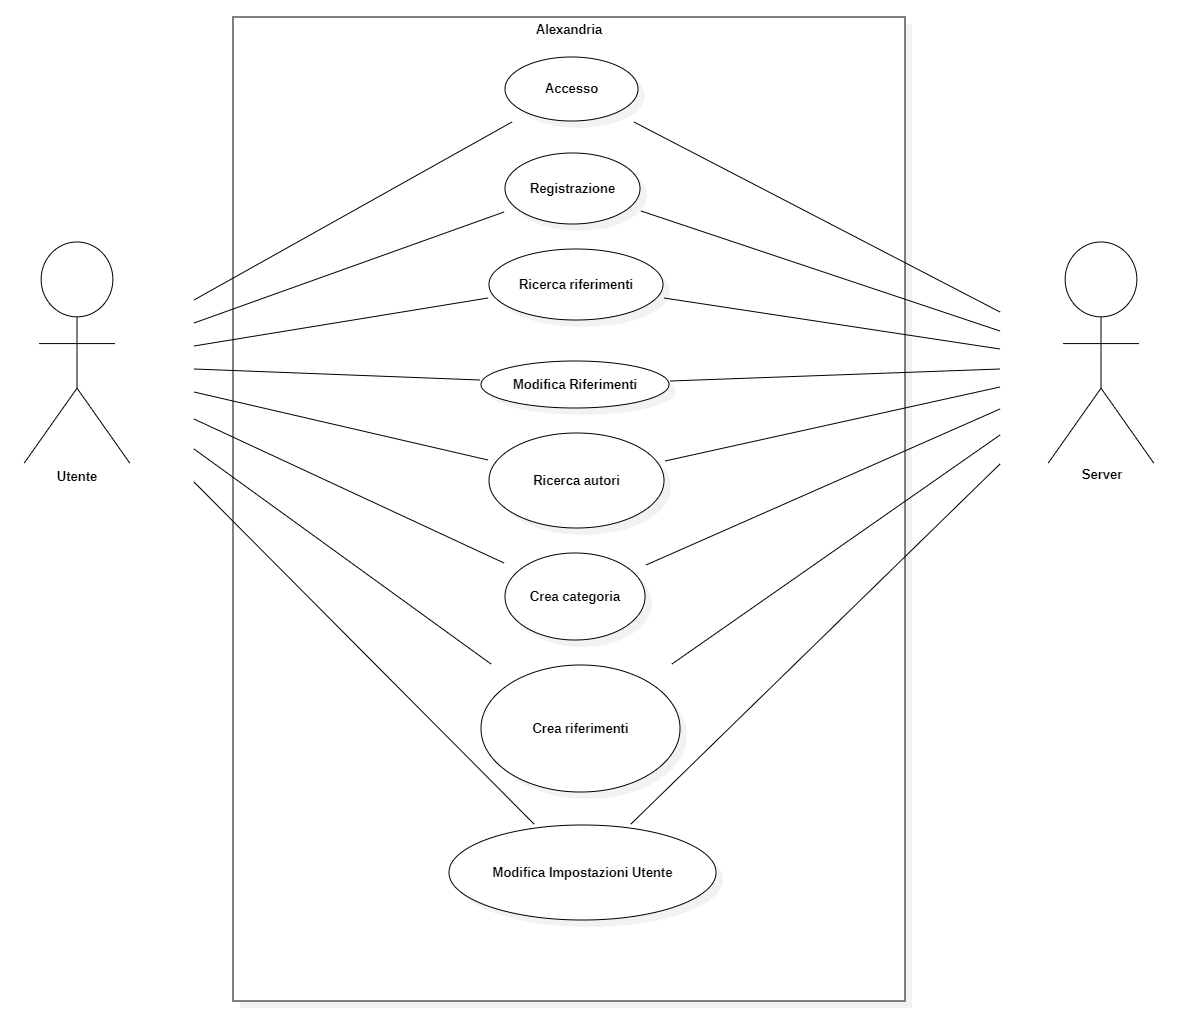
\includegraphics[width=.90\textwidth]{Immagini/Alexandria/useCase.png} 
        \end{center}
\newpage
Spiegazione dettagliata dei casi d'uso mostrati: 
\begin{itemize}
    \item Il caso d'uso \textit{Accesso} permette l'autenticazione di un utente, ovvero permette ad un utente di accedere al sistema inserendo le proprie credenziali (scelte dall'utente stesso durante la fase di registrazione).
    \item  Il caso d'uso \textit{Registrazione} permette di registrare un nuovo utente al sistema, scegliendo un proprio username, una propria password e una email.
    \item Il caso d'uso \textit{Ricerca Riferimenti} permette ad un utente di cercare un riferimento esistente nel sistema. Se inesistente, il sistema notifica l'utente dell'inesistenza del riferimento cercato, altrimenti permette di visualizzarlo. 
    \item Il caso d'uso \textit{Modifica Riferimenti} permette ad un utente di modificare un riferimento creato in precedenza, in particolare permette di modificare un \gls{attributo} inserito in precedenza,  potendo scegliere un nuovo valore. 
    \item  Il caso d'uso \textit{Ricerca autori} permette all'utente di ricercare un autore in particolare e tutte le sue opere pubblicate presenti nel sistema.
    \item Il caso d'uso \textit{Crea categoria} permette all'utente di creare una categoria e di poter scegliere un'eventuale \gls{sopra-categoria}.
    \item  Il caso d'uso \textit{Crea Riferimenti} permette ad un utente di creare un riferimento e di poterne assegnare gli attributi. 
    \item Infine, il caso d'uso \textit{Modifica Impostazioni utente} permette ad un utente di modificare tutte le informazioni inserite durante la fase di registrazione.
\end{itemize}
Tutte queste funzionalità richiedono un attore esterno, ovvero il Server, il quale permette di registrare ogni modifica al sistema. Sostanzialmente, senza di esso l'applicativo non può funzionare correttamente.


\raggedright{\section{Individuazione target degli utenti}}
Il target principale degli utenti sono coloro i quali intendono gestire e visualizzare i propri riferimenti bibliografici. Per tale motivo Alexandria permette la gestione e la visualizzazione affidabile dei riferimenti creati. In aggiunta, è possibile visualizzare i riferimenti degli altri utenti presenti nel sistema.
Un altro possibile target di utenti sono gli autori stessi dei riferimenti bibliografici, poiché possono gestire facilmente le proprie opere pubblicate e visualizzarne gli attributi.
Un altro target di utenti sono le case editrici che intendono gestire le varie edizioni dei propri riferimenti pubblicati. 
Considerando tutti i possibili utenti, il team si impegna di poter soddisfare tutte le esigenze degli usufruitori e di poter garantire un'eccellente usabilità e affidabilità del sistema.

\raggedright{\section{4 casi d'uso in particolare}}
\raggedright{\subsection{Caso d'uso: Ricerca Riferimenti}}

\begin{table}[H]    

\def\arraystretch{1.5}

\begin{tabularx}{\linewidth}{|l|X|X|X|}

  \hline Caso d'Uso 1 & \multicolumn{3} {l|}{Ricerca di un riferimento} \\ \hline Obiettivo & \multicolumn{3}{>{\hsize=\dimexpr 3\hsize+4\tabcolsep+2\arrayrulewidth\relax}X|}{%
    L'obiettivo principale è quello di ricercare uno o più riferimenti inserendo attributi specifici} \\
 \hline Precondizioni &
  \multicolumn{3}{l|}{L'utente deve essere stato correttamente registrato in precedenza.} \\
 \hline Condizioni di successo &
  \multicolumn{3}{l|}{L'utente trova e visualizza il riferimento desiderato} \\
 \hline Condizioni di fallimento &
  \multicolumn{3}{l|}{L'utente non trova il riferimento desiderato poiché inesistente} \\
 \hline Attore principale &
  \multicolumn{3}{l|}{Utente registrato} \\
 \hline Trigger & \multicolumn{3}{l|}{Utente preme su \textit{Ricerca} nella Homepage.} \\

  \hline \multirow{2}{*}{Descrizione} & Step & Attore & Sistema \\

  \cline{2-4} &  1 & Inserisce titolo del riferimento & \\
  \cline{2-4} &  2 & Seleziona uno dei \gls{tipi di riferimento} disponibili & \\
  \cline{2-4} &  3 &  & Seleziona i tipi di riferimento scelti \\
  \cline{2-4} &  4 & Cerca una categoria apposita &  \\
  \cline{2-4} &  5 &  & Mostra le categorie cercate dall'utente \\
  \cline{2-4} &  6 & Seleziona il \gls{tipo di ricerca} & \\
  \cline{2-4} &  7 & & Deselziona i tipi di ricerca non scelti dall'utente \\
  \cline{2-4} &  8 & Preme su ricerca & \\
  \cline{2-4} &  9 &  & Mostra frame \textit{Risultati ricerca} \\
  \cline{2-4} &  10 & Seleziona ordine ricerca & \\
  \cline{2-4} &  11 &  & Ordina ricerca per il tipo selezionato dall'utente \\
  \cline{2-4} &  12 & Seleziona un riferimento & \\
  \cline{2-4} &  13 &  & Mostra frame \textit{Visualizza Citazione}\\
   \hline Note & \multicolumn{3}{l|}{I nomi dei \textit{frame} provengono dai MockUp realizzati su Figma.} \\
 \hline

    \end{tabularx}
    \end{table}
    \newpage
    \begin{table}[H]
    \def\arraystretch{1.5}
    \begin{tabularx}{\linewidth}{|l|X|X|X|}
        
 \hline \multirow{2}{*}{Extensions A:  L'utente torna indietro} & Step &
  Attore & Sistema \\
 \cline{2-4} & D.1 a D.7 & Preme su \textit{Indietro} & \\
 \cline{2-4} &  A.1 &  & Mostra frame \textit{HomePage} \\
 \hline
  \multirow{2}{*}{Extension B: L'utente non inserisce il testo} & Step & Attore & Sistema \\

  \cline{2-4} & D.1 a D.7 & Utente preme su ricerca & \\
  \cline{2-4} & B.1 &  & Mostra tutti i riferimenti esistenti \\
 \hline
  \multirow{2}{*}{Extension C: Non esistono i riferimenti ricercati} & Step & Attore & Sistema \\

  \cline{2-4} & D.8 + D.9 & Utente preme su ricerca & \\
  \cline{2-4} & C.1  &  & Mostra frame \textit{Ricerca Vuota} \\
  \cline{2-4} & C.2  & L'utente preme su Crea &  \\
  \cline{2-4} & C.3  & & Mostra frame \textit{Crea Modifica Citazione}  \\
  \cline{2-4} & C.2  & L'utente seleziona Indietro &  \\
  \cline{2-4} & C.4  & & Ritorna a frame \textit{Ricerca}  \\

 \hline Note & \multicolumn{3}{l|}{I nomi dei \textit{frame} provengono dai MockUp realizzati su Figma.} \\
 \hline


\end{tabularx}

\end{table}

\raggedright{\subsection{Caso d'uso: Creazione Riferimento}}
\begin{tabularx}{\linewidth}{|l|X|X|X|}

  \hline Caso d'Uso 1 & \multicolumn{3} {l|}{Ricerca di un riferimento} \\ \hline Obiettivo & \multicolumn{3}{>{\hsize=\dimexpr 3\hsize+4\tabcolsep+2\arrayrulewidth\relax}X|}{%
    This is a very long line. Lorem ipsum dolor sit amet, consectetur
    adipiscing elit, sed do eiusmod tempor incididunt ut labore et
    dolore magna aliqua.  } \\
 \hline Precondizioni &
  \multicolumn{3}{l|}{} \\
 \hline Condizioni di successo &
  \multicolumn{3}{l|}{} \\
 \hline Condizioni di fallimento &
  \multicolumn{3}{l|}{} \\
 \hline Attore principale &
  \multicolumn{3}{l|}{} \\
 \hline Trigger & \multicolumn{3}{l|}{} \\

  \hline \multirow{2}{*}{Descrizione} & Step & Attore & Sistema \\

  \cline{2-4} & & & \\
 \hline \multirow{2}{*}{Extensions} & Step &
  Attore & Sistema \\
 \cline{2-4} & & & \\
 \hline
  \multirow{2}{*}{Sottovarianti} & Step & Attore & Sistema \\

  \cline{2-4} & & & \\
 \hline Nots & \multicolumn{3}{l|}{} \\
 \hline


\end{tabularx}

\raggedright{\subsection{Caso d'uso: Modifica propri Riferimenti}}
\begin{tabularx}{\linewidth}{|l|X|X|X|}

  \hline Caso d'Uso 1 & \multicolumn{3} {l|}{Ricerca di un riferimento} \\ \hline Obiettivo & \multicolumn{3}{>{\hsize=\dimexpr 3\hsize+4\tabcolsep+2\arrayrulewidth\relax}X|}{%
    This is a very long line. Lorem ipsum dolor sit amet, consectetur
    adipiscing elit, sed do eiusmod tempor incididunt ut labore et
    dolore magna aliqua.  } \\
 \hline Precondizioni &
  \multicolumn{3}{l|}{} \\
 \hline Condizioni di successo &
  \multicolumn{3}{l|}{} \\
 \hline Condizioni di fallimento &
  \multicolumn{3}{l|}{} \\
 \hline Attore principale &
  \multicolumn{3}{l|}{} \\
 \hline Trigger & \multicolumn{3}{l|}{} \\

  \hline \multirow{2}{*}{Descrizione} & Step & Attore & Sistema \\

  \cline{2-4} & & & \\
 \hline \multirow{2}{*}{Extensions} & Step &
  Attore & Sistema \\
 \cline{2-4} & & & \\
 \hline
  \multirow{2}{*}{Sottovarianti} & Step & Attore & Sistema \\

  \cline{2-4} & & & \\
 \hline Nots & \multicolumn{3}{l|}{} \\
 \hline


\end{tabularx}

\raggedright{\subsection{Caso d'uso: Crea Categoria}}
\begin{tabularx}{\linewidth}{|l|X|X|X|}

  \hline Caso d'Uso 1 & \multicolumn{3} {l|}{Ricerca di un riferimento} \\ \hline Obiettivo & \multicolumn{3}{>{\hsize=\dimexpr 3\hsize+4\tabcolsep+2\arrayrulewidth\relax}X|}{%
    L'obiettivo principale è quello di ricercare un determinato riferimento inserendo
    dettagli specifici.} \\
 \hline Precondizioni &
  \multicolumn{3}{l|}{} \\
 \hline Condizioni di successo &
  \multicolumn{3}{l|}{} \\
 \hline Condizioni di fallimento &
  \multicolumn{3}{l|}{} \\
 \hline Attore principale &
  \multicolumn{3}{l|}{} \\
 \hline Trigger & \multicolumn{3}{l|}{} \\

  \hline \multirow{2}{*}{Descrizione} & Step & Attore & Sistema \\

  \cline{2-4} & & & \\
 \hline \multirow{2}{*}{Extensions} & Step &
  Attore & Sistema \\
 \cline{2-4} & & & \\
 \hline
  \multirow{2}{*}{Sottovarianti} & Step & Attore & Sistema \\

  \cline{2-4} & & & \\
 \hline Nots & \multicolumn{3}{l|}{} \\
 \hline


\end{tabularx}

\raggedright{\section{MockUp Interfaccia grafica}}

\raggedright{\section{Valutazione dell'usabilità}}

\raggedright{\section{Classi, oggetti e relazioni d'analisi}}

\raggedright{\section{Diagrammi di Sequenza}}

\raggedright{\section{Prototipazione funzionale}}









